% Talk for the meeting with Dmitry Krotov, 2026-11-25.
% Compile:  sbatch compile_talk.sh     (one-CPU Slurm job; writes talk.pdf)
% All numbers: seed 1, 2,000 samples, Inception FID against the train split,
% from CODE_AND_PERFORMANCE.md (entries of 2026-11-21 to 2026-11-24).
\documentclass[aspectratio=169,10pt]{beamer}

\usepackage[T1]{fontenc}
\usepackage{helvet}
\usepackage{amsmath,amssymb,bm}
\usepackage{booktabs}
\usepackage{tikz}
\usetikzlibrary{calc}

% ---- look: the colours of the overview figure --------------------------------
\definecolor{ink}{HTML}{202326}
\definecolor{muted}{HTML}{65696D}
\definecolor{hair}{HTML}{B6B8BA}
\definecolor{cyan}{HTML}{477B8B}
\definecolor{globalcol}{HTML}{7B5C8D}
\definecolor{coarsecol}{HTML}{B4664B}
\definecolor{finecol}{HTML}{C29A38}

\usetheme{default}
\setbeamertemplate{navigation symbols}{}
\setbeamercolor{normal text}{fg=ink,bg=white}
\setbeamercolor{frametitle}{fg=cyan}
\setbeamercolor{structure}{fg=cyan}
\setbeamercolor{alerted text}{fg=coarsecol}
\setbeamerfont{frametitle}{series=\bfseries,size=\large}
\setbeamertemplate{itemize item}{\color{cyan}\rule[0.25ex]{0.5ex}{0.5ex}}
\setbeamertemplate{itemize subitem}{\color{muted}--}
\setbeamertemplate{footline}{\hfill{\color{muted}\scriptsize\insertframenumber\,/\,\inserttotalframenumber}\hspace{0.6em}\vspace{0.5em}}
\setbeamersize{text margin left=0.8cm,text margin right=0.8cm}

\newcommand{\x}{\bm{x}}
\newcommand{\gen}{\mathcal{L}}
\DeclareMathOperator{\Cov}{Cov}
\newcommand{\src}[1]{{\color{muted}\scriptsize #1}}
\newcommand{\key}[1]{{\color{cyan}\bfseries #1}}

% image strip with row labels: \strip{file}{height}{number of rows}{label 1,label 2,...}
\newcommand{\strip}[4]{%
  \begin{tikzpicture}
    \node[inner sep=0,anchor=south west] (img) at (0,0) {\includegraphics[height=#2]{img/#1}};
    \foreach \lab [count=\i] in {#4} {
      \pgfmathsetmacro{\f}{(\i-0.5)/#3}
      \node[anchor=east,font=\scriptsize,text=ink] at ($(img.north west)!\f!(img.south west)+(-0.12,0)$) {\lab};
    }
  \end{tikzpicture}}

\title{A dense associative memory as a physical diffusion model}
\subtitle{trained templates, fast hidden units, and a local learning rule with a single phase}
\author{Cyrill B\"osch}
\date{Discussion with Dmitry Krotov, 25 November 2026}

\begin{document}

% ------------------------------------------------------------------------------
\begin{frame}[plain]
  \vspace{0.8cm}
  {\color{cyan}\LARGE\bfseries A \textit{trained} dense associative memory\\[2pt] as a physical diffusion model\par}
  \vspace{0.35cm}
  {\large trained templates, fast hidden units,\\ and a local learning rule with a single phase\par}
  \vspace{1.0cm}
  {Cyrill B\"osch, Ryan Adams\par}
  \vspace{0.15cm}
  {\color{muted}\small Discussion with Dmitry Krotov, 25 November 2026\par}
  \vspace{0.9cm}
  {\color{muted}\footnotesize All results are simulations. Numbers: one seed, 2{,}000 samples, Inception FID.\par}
\end{frame}

% ------------------------------------------------------------------------------
\begin{frame}{The system in one picture}
  \centering
  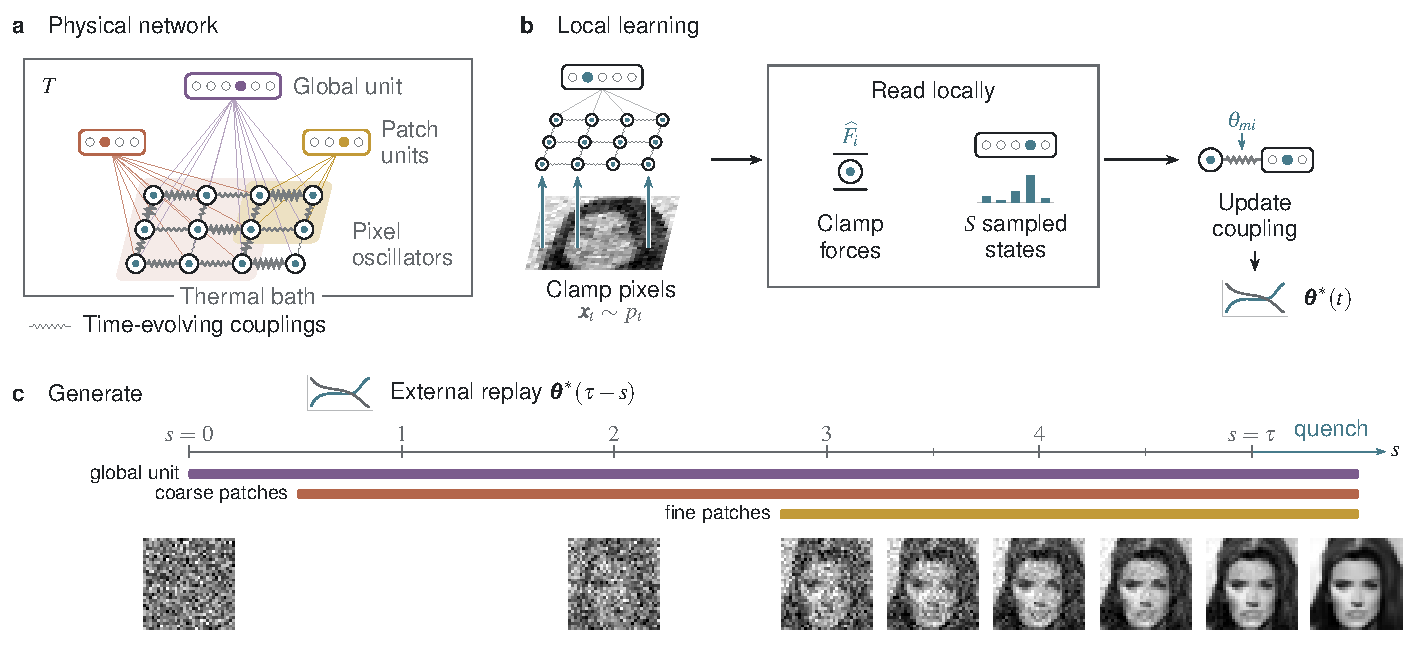
\includegraphics[width=\textwidth]{img/overview.pdf}

  % \vspace{0.1cm}
  % \begin{columns}[T,onlytextwidth]
  %   \column{0.32\textwidth}\footnotesize
  %     \key{a}\; Pixels are oscillators in a thermal bath. Fast hidden Potts units couple to all
  %     pixels or to one patch.
  %   \column{0.32\textwidth}\footnotesize
  %     \key{b}\; Learning: clamp the pixels to a noised image, read the hidden units,
  %     update each coupling.
  %   \column{0.32\textwidth}\footnotesize
  %     \key{c}\; Generation: replay the learned couplings in reverse time, then switch
  %     the bath off.
  % \end{columns}
\end{frame}

% ------------------------------------------------------------------------------
\begin{frame}{Overview}
  \begin{itemize}\setlength{\itemsep}{9pt}
    \item \key{Model.}  The \textit{time dependent} energy of a dense associative memory at finite temperature (bipartite graph) + slow visible units.\\
    \item \key{Learning rule.} Local, and evaluated in \emph{one phase} with the pixels
      (Voltage-) clamped to data:  Measure forces (currents) and hidden statistics\\
      No free-running phase and no nudged phase.
    \item \key{Results.} Trained from 16 sampled hidden states per unit and image, the
      model generates digits, garments and faces, 1 to 3 FID above training with exact
      hidden averages.
    
    \item \key{Generation.} Stochastic (SDE; shown) or deterministic (probability flow ODE).
  \end{itemize}
\end{frame}

% ------------------------------------------------------------------------------
\begin{frame}{Starting point: diffusion as physical dynamics}
  \vspace{0.2cm}
  \textbf{Noising} = relaxation of uncoupled oscillators at temperature $T$
  \[
    \mathrm{d}\x=-\x\,\mathrm{d}t+\sqrt{2T}\,\mathrm{d}W ,\qquad t\in[0,\tau]
  \]
  \vspace{0.1cm}

  \textbf{Generation} = Langevin dynamics of the pixels while the couplings are driven
  \[
    \mathrm{d}\x=\bigl[\x-2\nabla F_{\tau-s}(\x)\bigr]\mathrm{d}s+\sqrt{2T}\,\mathrm{d}W
  \]
  \vspace{0.1cm}

  $F_t(\x)$ is the \textbf{free energy} of the pixels after the fast hidden units $h$ are summed out:
  \[
    e^{-F_t(\x)/T}=\sum_{h}e^{-E_t(\x,h)/T}
  \]
\end{frame}

% ------------------------------------------------------------------------------
\begin{frame}{The model: pixels plus one layer of fast hidden units}
  \textbf{Joint energy} ($y^{u}$: one-hot state of Potts unit $u$; $\sigma_i=\pm1$; no hidden--hidden coupling)
  {\small
  \[
    E_t(\x,y,\sigma)=E^{\mathrm v}_t(\x)-\sum_u\sum_{m=1}^{K_u} y^{u}_{m}\,a^{u}_{m}(\x,t)-\sum_i\sigma_i\bigl(\nu_i(t)+w_i(t)\,x_i\bigr),
  \]
  \vspace{-0.3cm}
  \[
    a^{u}_{m}(\x,t)=b^{u}_{m}(t)+\!\sum_{i\in\mathcal P_u}\!\bigl(W^{u}_{mi}(t)\,x_i+Q^{u}_{mi}(t)\,x_i^{2}\bigr)
  \]}
  \vspace{-0.05cm}

  {\footnotesize\color{muted} All couplings depend on the noise level $t$. From here on the $t$ is not written.}
  \vspace{0.05cm}


  \textbf{Fast hidden units sum out exactly.} The pixels move in the free energy
  \[
    F_t(\x)=E^{\mathrm v}_t(\x)
      \;-\;T\sum_u\log\sum_{m=1}^{K_u}e^{a^{u}_{m}(\x)/T}
      \;-\;T\sum_i\log2\cosh\frac{\nu_i+w_ix_i}{T}
  \]
  \vspace{-0.2cm}
  \begin{columns}[T,onlytextwidth]
    \column{0.47\textwidth}\small
      \begin{itemize}
        \item {\color{globalcol}\bfseries Global unit}: $K$ states, all pixels
        \item {\color{coarsecol}\bfseries Coarse} and {\color{finecol}\bfseries fine patch units}:
          $M=64$ states, one unit per overlapping patch
        \item Per-pixel bistable unit $\sigma_i$
      \end{itemize}
    \column{0.49\textwidth}\small
      \begin{itemize}
        \item $E^{\mathrm v}$: on-site well per pixel, springs to the 8 neighbours
        \item The second term is your log-sum-exp energy, at temperature $T$
          \src{Krotov \& Hopfield 2021}
      \end{itemize}
  \end{columns}
\end{frame}

% ------------------------------------------------------------------------------
\begin{frame}{One Potts unit: what it is and what it does to the pixels}
  \begin{columns}[T,onlytextwidth]
    \column{0.50\textwidth}
      A Potts unit has $K$ states; exactly one is active.
      \vspace{0.15cm}

      \textbf{What it sees:} the field of each state,
      \[
        a_m(\x)=b_m+W_m\!\cdot\!\x+Q_m\!\cdot\!\x^{2}
      \]
      \textbf{How it responds} (fast, thermal): time spent in state $m$
      \[
        p_m(\x)=\frac{e^{a_m/T}}{\sum_k e^{a_k/T}}
      \]
      \textbf{What the pixels feel:} the time-averaged force
      \[
        -\nabla F\;\ni\;\sum_m p_m\,G_m,\qquad G_m=W_m+2Q_m\!\circ\!\x
      \]
    \column{0.46\textwidth}
      \vspace{0.2cm}
      \begin{itemize}\setlength{\itemsep}{8pt}
        \item States are mutually exclusive (stochastic winner-take-all).
        \item Given the image, all hidden units are independent. They talk to each other
          only through the pixels they share.
      \end{itemize}
  \end{columns}
\end{frame}

% ------------------------------------------------------------------------------
\begin{frame}{What $W$, $Q$ and $b$ do to a pixel}
  \begin{columns}[T,onlytextwidth]
    \column{0.47\textwidth}
      With state $m$ active, pixel $i$ sits in the well
      \begin{align*}
        &\tfrac{k_i}{2}x_i^{2}-W_{mi}x_i-Q_{mi}x_i^{2}\\
        &\qquad=\tfrac{\kappa_{mi}}{2}\,(x_i-\xi_{mi})^{2}+\text{const}
      \end{align*}
      \[
        \kappa_{mi}=k_i-2Q_{mi},\qquad \xi_{mi}=\frac{W_{mi}}{\kappa_{mi}}
      \]
      \vspace{-0.2cm}
      \begin{itemize}\setlength{\itemsep}{5pt}
        \item $W$: \textbf{where} the state pulls the pixel (the template $\xi_m$)
        \item $Q$: \textbf{how tightly} it holds it (stiffness; width $\sqrt{T/\kappa}$)
        \item $b$: how often the state is used
      \end{itemize}
    \column{0.50\textwidth}
      \centering
      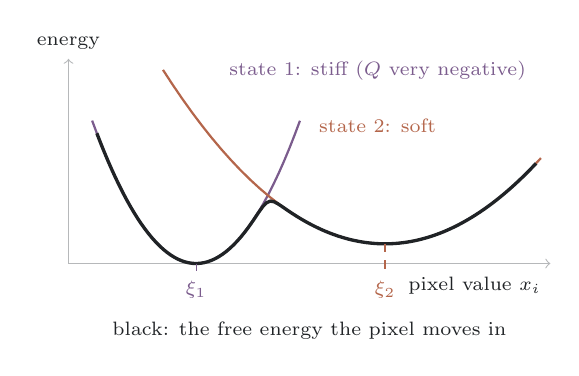
\begin{tikzpicture}[x=1.2cm,y=1.0cm]
        \draw[hair,->] (-2.35,0)--(2.75,0);
        \node[ink,font=\scriptsize,anchor=north east] at (2.75,-0.05) {pixel value $x_i$};
        \draw[hair,->] (-2.35,0)--(-2.35,2.6) node[above,ink,font=\scriptsize]{energy};
        % state 1: stiff, centred at -1; state 2: soft, centred at +1
        \draw[globalcol,thick,domain=-2.1:0.1,samples=40] plot (\x,{1.5*(\x+1)*(\x+1)});
        \draw[coarsecol,thick,domain=-1.35:2.65,samples=40] plot (\x,{0.4*(\x-1)*(\x-1)+0.25});
        \draw[ink,very thick,domain=-2.05:2.6,samples=120]
          plot (\x,{min(1.5*(\x+1)*(\x+1),0.4*(\x-1)*(\x-1)+0.25)
                    -0.12*ln(1+exp(-min(abs(1.5*(\x+1)*(\x+1)-0.4*(\x-1)*(\x-1)-0.25)/0.12,12)))});
        \node[globalcol,font=\scriptsize,align=left,anchor=west] at (-0.75,2.45) {state 1: stiff ($Q$ very negative)};
        \node[coarsecol,font=\scriptsize,align=left,anchor=west] at (0.2,1.75) {state 2: soft};
        \draw[globalcol,dashed] (-1,0)--(-1,-0.1) node[below,font=\scriptsize]{$\xi_1$};
        \draw[coarsecol,dashed] (1,0.25)--(1,-0.1) node[below,font=\scriptsize]{$\xi_2$};
        \node[ink,font=\scriptsize] at (0.2,-0.85) {black: the free energy the pixel moves in};
      \end{tikzpicture}

      \vspace{0.1cm}
      {\footnotesize Without $Q$ all templates share one width.\\
       On faces: FID 34 without $Q$, 22 with it \src{(earlier, larger model)}}
  \end{columns}
\end{frame}

% ------------------------------------------------------------------------------
\begin{frame}{Why each part is there}
  \footnotesize
  \setlength{\tabcolsep}{5pt}
  \begin{tabular}{@{}p{3.1cm}p{5.5cm}p{4.9cm}@{}}
    \toprule
    Part & What it does to the pixels & Evidence (FID, lower is better) \\
    \midrule
    On-site well & keeps each pixel bounded & quartic $\to$ harmonic: $20.2\to21.0$ \\[3pt]
    Springs to 8 neighbours & correlate neighbouring pixels; given the hidden states the pixels
      are otherwise independent & without: same faces, with grain; $20.2\to25.8$ \\[3pt]
    {\color{globalcol}Global Potts unit} & long-range agreement: which class, which layout &
      MNIST, $K=16\to784$: $14.4\to10.0$; faces: $20.2\to19.4$ \\[3pt]
    {\color{coarsecol}Patch} {\color{finecol}Potts units} & local structure; $M^{U}$ joint states, so
      images are composed, not looked up & faces without patch units: 104; with: 22
      \src{(earlier model)} \\[3pt]
    Bistable unit per pixel & an on-site double well (ink or background) & kept from the first
      models; not ablated here \\[3pt]
    Quadratic coupling $Q$ & a stiffness per state and pixel & faces: $34\to22$ \src{(earlier model)} \\[3pt]
    All hidden units & the content & pixels only: 218 \\
    \bottomrule
  \end{tabular}

  \vspace{0.25cm}
  {\footnotesize CelebA $32\times32$ unless stated. The coarse patch set acts for $t\le4.49$, the fine one
  for $t\le2.22$ (of $\tau=5$): coarse structure forms at higher noise.}
\end{frame}

% ------------------------------------------------------------------------------
\begin{frame}{Relation to your work: stored patterns against trained templates}
  \begin{columns}[T,onlytextwidth]
    \column{0.52\textwidth}
      \textbf{The model class contains the memory that stores the data.}\\[3pt]
      The exact score of a noised training set $\{\x_n\}$ is one Potts unit with one state
      per image:
      \[
        W_n=\frac{e^{-t}\x_n}{\gamma_t},\quad
        Q_{ni}=-\frac{1}{2\gamma_t},\quad
        b_n=-\frac{e^{-2t}\lVert\x_n\rVert^{2}}{2\gamma_t}
      \]
      with $\gamma_t=1-e^{-2t}$. As a generator it returns the training set.
      \src{Hoover et al.\ 2023; Ambrogioni 2024; Pham, Raya, Negri, Zaki, Ambrogioni, Krotov 2026}

      \vspace{0.25cm}
      \textbf{We keep $K\ll N$ states and train $b$, $W$, $Q$} at every noise level by score
      matching, and add local templates on patches.
    \column{0.44\textwidth}
      \vspace{0.1cm}
      \small
      \begin{tabular}{@{}lc@{}}
        \toprule
        CelebA $32\times32$ \src{(earlier model)} & FID \\
        \midrule
        templates held at data prototypes & 147 \\
        templates learned, no $Q$ & 34 \\
        templates learned, with $Q$ & 22 \\
        \bottomrule
      \end{tabular}

      \vspace{0.4cm}
      \begin{itemize}\setlength{\itemsep}{5pt}
        \item Faces: 16 global templates for 163{,}000 images.
        \item Templates are \emph{initialised} from $k$-means prototypes, then learned.
        \item Are these ``memories'' in your sense? Each noise level has its own set, and a
          generated image is a composition, not one retrieved template.
        \item I have not measured memorisation; samples are not copies of their nearest
          training images.
      \end{itemize}
  \end{columns}
\end{frame}

% ------------------------------------------------------------------------------
\begin{frame}{Generation is a protocol on the device}
  \begin{columns}[T,onlytextwidth]
    \column{0.50\textwidth}
      \begin{enumerate}\setlength{\itemsep}{7pt}
        \item \textbf{Start} from the thermal state $\mathcal N(0,TI)$.
        \item \textbf{Drive}: replay the couplings $\theta_{\tau-s}$ while the bath supplies the
          noise. The pixels move in $2F_{\tau-s}-\tfrac12\lVert\x\rVert^{2}$.
        \item {\color{coarsecol}Coarse} patches switch on at $s\approx0.5$,
          {\color{finecol}fine} ones at $s\approx2.8$.
        \item \textbf{Quench}: switch the bath off, $\dot{\x}=-\nabla F_0(\x)$, for a short time.
      \end{enumerate}
    \column{0.46\textwidth}
      \vspace{0.1cm}
      \begin{itemize}\setlength{\itemsep}{7pt}
        \item The hidden units are neither controlled nor read during generation.
        \item 100 stored coupling sets, interpolated linearly in time.
        \item The factor 2: for the hidden units it needs two copies of each unit at
          temperature $T$, or a gain of 2 on their force.
        \item Deterministic variant: the probability-flow ODE (results below).
      \end{itemize}
  \end{columns}
\end{frame}

% ------------------------------------------------------------------------------
\begin{frame}{Learning rule, part 1: the gradient is a response to release}
  Score matching at one noise level, written with forces
  ($\bm\psi=\nabla F_t$ is the force a clamp must supply to hold the pixels):
  \[
    J_t=\Bigl\langle-\frac{\Delta F_t}{T}+\frac{\lVert\nabla F_t\rVert^{2}}{2T^{2}}\Bigr\rangle_{\x\sim p_t}
    \qquad\Longrightarrow\qquad
    \boxed{\;\partial_\theta J_t=-\frac{1}{T^{2}}\bigl\langle\gen\,\partial_\theta F_t\bigr\rangle,
    \qquad \gen=T\Delta-\bm\psi\!\cdot\!\nabla\;}
  \]
  \begin{itemize}\setlength{\itemsep}{6pt}
    \item $\gen$ is the generator of the pixels' own Langevin dynamics in $F_t$.
    \item $\partial_\theta F_t$ is the Hebbian term of a Boltzmann machine: $-p_m$ for a bias,
      $-p_mx_i$ for a coupling.
    \item So: \emph{learning has converged when the Hebbian terms are stationary under the model's
      own dynamics started from data.}
    \item One could measure this by releasing the pixels briefly (contrastive divergence with
      one short step). That is a difference of two noisy readings. We evaluate
      $\gen\,\partial_\theta F_t$ at the clamp instead.
  \end{itemize}
\end{frame}

% ------------------------------------------------------------------------------
\begin{frame}{Learning rule, part 2: one phase, read from fluctuations}
  \begin{columns}[T,onlytextwidth]
    \column{0.50\textwidth}
      For a Potts unit, with $\delta G_k=G_k-\bar G$ the excess force of state $k$:
      \[
        \gen\,p_m=\frac{1}{T}\,\Cov_k\bigl(\delta_{km},\,\phi_k\bigr)
      \]
      \[
        \phi_k=\delta G_k\!\cdot\!\bigl(\delta G_k-\bm\psi\bigr)+2T\textstyle\sum_iQ_{ki}
      \]
      \textbf{Per read} of the hidden unit (found in state $k$), only that state's couplers
      change:
      \[
        \Delta W_{ki}\;\propto\;-\frac{x_i(\phi_k-\bar\phi)}{T^{3}}-\frac{2\,\delta G_{ki}-\psi_i}{T^{2}}
      \]
    \column{0.46\textwidth}
      \vspace{0.15cm}
      \begin{itemize}\setlength{\itemsep}{7pt}
        \item \textbf{One experiment per image}: pixels held at the noised data point,
          everything is read there.
        \item No free-running phase, because it is a different objective: score matching
          compares forces at the data and has no partition function.
        \item It does need how the hidden unit responds when the pixels move. A thermal
          unit shows that in its \emph{fluctuations}, so the clamp is never displaced.
        \item Price: thermal hidden units are required; a $1/S$ bias from $S$ reads,
          removed by a jackknife.
      \end{itemize}
  \end{columns}

  \vspace{0.15cm}
  {\footnotesize\color{muted} Checked against automatic differentiation. In the simulations only the hidden
  states are sampled; forces and sums are exact.}
\end{frame}

% ------------------------------------------------------------------------------
\begin{frame}{Result 1: training from sampled hidden states}
  \begin{columns}[T,onlytextwidth]
    \column{0.60\textwidth}
      \footnotesize
      \setlength{\tabcolsep}{4pt}
      \begin{tabular}{@{}lcccc@{}}
        \toprule
        FID & MNIST & Fashion & Faces\,32 & Faces\,64 \\
        \midrule
        exact hidden averages & 10.0 & 21.3 & 20.2 & 43.2 \\
        sampled, $S=64$ reads & 11.4 & 23.4 & 21.2 & 46.0 \\
        sampled, $S=16$ reads & 11.8 & 22.9 & 21.2 & 46.6 \\
        \midrule
        \multicolumn{5}{@{}l}{\emph{with two corrector steps per noise level}} \\
        exact hidden averages & 9.2 & 21.8 & 20.0 & 38.2 \\
        sampled, $S=64$ reads & 9.8 & 23.5 & 20.2 & 41.3 \\
        sampled, $S=16$ reads & 10.2 & 23.5 & 20.5 & 41.1 \\
        \midrule
        real test images (floor) & 3.7 & 7.2 & 6.4 & 5.9 \\
        \bottomrule
      \end{tabular}

      \vspace{0.15cm}
      {\scriptsize\color{muted} Global unit: $K=784$ for MNIST and Fashion-MNIST, $K=16$ for faces (CelebA, grey).}
    \column{0.37\textwidth}
      \small
      \begin{itemize}\setlength{\itemsep}{7pt}
        \item Sampled training is \textbf{1 to 3 FID above exact}. Close, not equal.
        \item \textbf{16 reads are as good as 64.} The gap is not set by the number of reads;
          its origin is not isolated.
        \item The gap grows with resolution: 1.0 at $32\times32$, about 3 at $64\times64$.
        \item $64\times64$ is far from the floor.
      \end{itemize}
  \end{columns}
\end{frame}

% ------------------------------------------------------------------------------
\begin{frame}{The same model is learned: same noise, same faces}
  \centering
  \strip{strip_c32.png}{2.65cm}{4}{real,exact,sampled $S=64$,sampled $S=16$}

  \vspace{0.15cm}
  \strip{strip_c64.png}{2.65cm}{4}{real,exact,sampled $S=64$,sampled $S=16$}

  \vspace{0.1cm}
  {\footnotesize CelebA $32\times32$ (top) and $64\times64$ (bottom). Each column: the same initial noise
  and noise path. The three models start training from the same initial templates.}
\end{frame}

% ------------------------------------------------------------------------------
\begin{frame}{Uncurated samples, models trained from $S=64$ sampled states}
  \centering
  \includegraphics[width=0.325\textwidth]{img/grid_mnist.png}\hfill
  \includegraphics[width=0.325\textwidth]{img/grid_fashion.png}\hfill
  \includegraphics[width=0.325\textwidth]{img/grid_c32.png}

  \vspace{0.15cm}
  {\footnotesize MNIST (FID 11.4), Fashion-MNIST (23.4), CelebA $32\times32$ (21.2). First 100 of 2{,}000
  samples. Defects: some malformed digits; faces have less contrast than the data.}
\end{frame}

% ------------------------------------------------------------------------------
\begin{frame}{CelebA $64\times64$}
  \begin{columns}[c,onlytextwidth]
    \column{0.46\textwidth}
      \centering
      \includegraphics[height=6.3cm]{img/grid_c64.png}
    \column{0.50\textwidth}
      \begin{itemize}\setlength{\itemsep}{8pt}
        \item Same architecture, patch sizes doubled; $K=16$.
        \item Trained from $S=64$ sampled states: FID 46.0 (exact 43.2; with corrector 41.3 and 38.2).
        \item Plausible, varied faces; smudgy backgrounds, a few distorted faces, low contrast.
        \item Sampled training took 19 to 23 hours on one GPU.
      \end{itemize}
  \end{columns}
\end{frame}

% ------------------------------------------------------------------------------
\begin{frame}{Result 2: the global unit carries the class}
  \begin{columns}[T,onlytextwidth]
    \column{0.37\textwidth}
      \small
      \begin{tabular}{@{}lccc@{}}
        \toprule
        Global unit & MNIST & Fashion & Faces \\
        \midrule
        $K=16$  & 14.4 & 26.0 & 20.2 \\
        $K=128$ & 12.0 & 23.5 & -- \\
        $K=784$ & 10.0 & 21.3 & 19.4 \\
        \bottomrule
      \end{tabular}

      \vspace{0.3cm}
      \begin{itemize}\setlength{\itemsep}{5pt}
        \item Ten classes: $K$ matters (4 to 5 FID).
        \item Faces: it hardly does (0.8).
        \item At $K=16$ digits have clean strokes, but 28\% are not a clear digit
          (17\% at $K=784$, 2\% for real digits).
      \end{itemize}
    \column{0.60\textwidth}
      \centering
      \strip{strip_mnist_K10.png}{3.2cm}{5}{real,earlier model,$K=16$,$K=128$,$K=784$}

      \vspace{0.2cm}
      \raggedright\small
      \textbf{My reading.} Patch units agree only through shared pixels, hence locally.
      Which of ten classes an image is, is a global decision and needs mutually exclusive
      templates per class. Aligned faces are one class with a fixed layout.\\[3pt]
      \emph{The number of global memories follows the number of global modes of the data,
      not the number of images.}
  \end{columns}
\end{frame}

% ------------------------------------------------------------------------------
\begin{frame}{Result 3: what the visible network contributes}
  \begin{columns}[T,onlytextwidth]
    \column{0.64\textwidth}
      \centering
      \strip{strip_springs10.png}{4.1cm}{6}{real,full model,linear on-site,no springs,linear + no springs,pixels only}
    \column{0.34\textwidth}
      \footnotesize
      \begin{tabular}{@{}lcc@{}}
        \toprule
        Faces\,32, FID & springs & none \\
        \midrule
        quartic on-site & 20.2 & 25.8 \\
        linear on-site  & 21.0 & 27.4 \\
        \midrule
        no hidden units & 218 & \\
        \bottomrule
      \end{tabular}

      \vspace{0.3cm}
      \begin{itemize}\setlength{\itemsep}{5pt}
        \item The hidden units carry the content.
        \item The springs remove grain; the faces stay the same.
        \item A visible network that is linear throughout costs 0.8 FID.
        \item Without springs the device is purely bipartite, as your circuit.
      \end{itemize}
  \end{columns}
\end{frame}

% ------------------------------------------------------------------------------
\begin{frame}{The sampler: noise, quench, and the probability-flow ODE}
  \begin{columns}[T,onlytextwidth]
    \column{0.62\textwidth}
      \centering
      \strip{strip_ode10.png}{3.6cm}{5}{real,exact: SDE,exact: ODE,sampled: SDE,sampled: ODE}

      \vspace{0.1cm}
      {\footnotesize Same initial noise per column. SDE and ODE end in different faces; exact and
      sampled training agree within each sampler.}
    \column{0.36\textwidth}
      \footnotesize
      \setlength{\tabcolsep}{4pt}
      \begin{tabular}{@{}lcc@{}}
        \toprule
        Faces\,32, FID & exact & $S=64$ \\
        \midrule
        reverse SDE, as sampled & 76.7 & 79.6 \\
        + quench & 20.2 & 21.2 \\
        + corrector and quench & 20.0 & 20.2 \\
        ODE + quench & 22.1 & 22.9 \\
        \bottomrule
      \end{tabular}

      \vspace{0.25cm}
      \begin{itemize}\setlength{\itemsep}{4pt}
        \item The quench removes the thermal noise of the pixels.
        \item The deterministic ODE costs about 2 FID: flatter, more uniform faces.
      \end{itemize}
  \end{columns}
\end{frame}

% ------------------------------------------------------------------------------
\begin{frame}{Probability-flow ODE samples}
  \centering
  \begin{columns}[c,onlytextwidth]
    \column{0.36\textwidth}
      \centering
      \includegraphics[height=5.3cm]{img/grid_c32_sde.png}\\[2pt]
      {\footnotesize reverse SDE + quench (FID 20.2)}
    \column{0.36\textwidth}
      \centering
      \includegraphics[height=5.3cm]{img/grid_c32_ode.png}\\[2pt]
      {\footnotesize probability-flow ODE + quench (FID 22.1)}
    \column{0.25\textwidth}
      \small
      \begin{itemize}\setlength{\itemsep}{6pt}
        \item CelebA $32\times32$, exact training, same initial noise.
        \item ODE: no noise source for the pixels during generation.
        \item Faces are flatter (more mid-grey) and more alike.
      \end{itemize}
  \end{columns}
\end{frame}

% ------------------------------------------------------------------------------
\begin{frame}{Time dependence: needed, and the main cost}
  \begin{columns}[T,onlytextwidth]
    \column{0.48\textwidth}
      \textbf{One landscape is not enough.}
      \begin{itemize}\setlength{\itemsep}{5pt}
        \item Langevin dynamics under the final energy $F_0$ alone, from noise, up to 5 times the
          protocol's duration: every chain ends in an almost blank image
          \src{(earlier MNIST model)}.
        \item The final landscape has no path from noise to data. The sequence of landscapes
          provides it.
        \item Parallel to your finite-temperature result: higher-order memories fail to
          retrieve far from every memory?
          \src{Rooke, Krotov, Balasubramanian, Wolpert 2026}
      \end{itemize}
    \column{0.48\textwidth}
      \textbf{100 coupling sets is a lot.}
      \begin{itemize}\setlength{\itemsep}{5pt}
        \item Replacing them after training by 5 (global) and 9 (per patch set), interpolated:
          faces $21.2\to23.7$ at $32\times32$, $46.0\to47.6$ at $64\times64$.
        \item On MNIST and Fashion-MNIST the same reduction fails (FID 234 and 88).
        \item A ``physical'' corrector, a fixed dwell at each noise level, does not help
          (20.3 to 21.5 against 20.2 without).
        \item Alternative: one energy, trained with a negative phase
          \src{Liao, Kornblith, Ren, Fleet, Hinton 2022}.
      \end{itemize}
  \end{columns}
\end{frame}

% ------------------------------------------------------------------------------
\begin{frame}{Towards hardware: your circuit, and what this model adds}
  \begin{columns}[T,onlytextwidth]
    \column{0.48\textwidth}
      \textbf{What exists} \src{Bacvanski, You, Hopfield, Krotov, arXiv 2512.15002}
      \begin{itemize}\setlength{\itemsep}{5pt}
        \item Visible and hidden neurons joined by one resistive crossbar, used in both
          directions.
        \item Softmax over the hidden neurons; hidden neurons about ten times faster.
        \item The visible neurons then move in the log-sum-exp energy: one of our Potts units in
          the deterministic limit, with stored weights.
      \end{itemize}
      \vspace{0.1cm}
      {\footnotesize\color{muted} My reading of your paper; please correct me.}
    \column{0.48\textwidth}
      \textbf{What this model needs beyond it}
      \begin{itemize}\setlength{\itemsep}{5pt}
        \item Noise: a bath for the pixels, and hidden units that \emph{fluctuate}
          (the rule reads their fluctuations).
        \item Couplings that change in time during generation.
        \item The quadratic couplings $Q$, and couplings of both signs.
        \item Read-out: the clamp force = the current each clamp supplies (a column read); the
          active state; one sum per hidden state (a row read). Then an
          update of one row of the array.
        \item Two copies of each hidden unit during generation (the factor 2).
      \end{itemize}
  \end{columns}
\end{frame}

% ------------------------------------------------------------------------------
\begin{frame}{What is not shown, and what is weak}
  \begin{itemize}\setlength{\itemsep}{7pt}
    \item \textbf{Simulation only}, in the limit of fast hidden units. Only the hidden states are
      sampled; forces and sums are exact, without read noise. No finite switching rate, no
      coupling precision.
    \item \textbf{One seed, 2{,}000 samples.} Seeds and larger sample sets are next.
    \item \textbf{FID is a coarse instrument here.} On MNIST it follows stroke texture more than
      digit identity. I do not rank against FIDs from other papers (protocols not stated).
    \item \textbf{Size}: 2 to 4 million couplings per noise level, times 100 noise levels. Per
      noise level this is the size of a Gaussian--Bernoulli RBM that generates MNIST.
    \item \textbf{Grey images}, at most $64\times64$; contrast too low; quality at $64\times64$ far
      from the floor.
    \item \textbf{The gap} between sampled and exact training (1 to 3 FID) is not explained.
    \item Preliminary, not in the tables: bistable units on the springs between pixels improve
      faces from 20.2 to about 18.4.
  \end{itemize}
\end{frame}

% ------------------------------------------------------------------------------
\begin{frame}{Where I would value your opinion}
  \begin{enumerate}\setlength{\itemsep}{6pt}
    \item \textbf{Framing.} Is ``a thermal, time-dependent dense associative memory with trained
      templates'' the right way to describe this? What would you want to see before calling it
      that?
    \item \textbf{Memorisation and generalisation.} With $K\ll N$ trained templates per noise
      level, where does this sit in your picture? Which diagnostic would you trust?
    \item \textbf{Global memories and classes.} $K$ matters for ten classes and not for faces.
      Is there a capacity argument behind this?
    \item \textbf{One energy or many.} Can the time dependence be reduced, for example to a
      schedule acting on one set of memories?
    \item \textbf{Hardware.} What would your circuit need for stochastic hidden units, signed and
      time-dependent couplings, and $Q$?
    \item \textbf{Thermodynamics.} The work and entropy production of the generation protocol.
  \end{enumerate}
  \vspace{0.25cm}
  {\color{cyan}\bfseries Plan:} a short paper for ICML (deadline 22 January 2027), on arXiv before.
  {\bfseries I would be glad to have you as a co-author.}
\end{frame}

\end{document}
